\section{Potential benefits of ray tracing}
Going away from the current rasterization-based rendering pipeline and instead using ray tracing to render the scene has many potential benefits.

\subsection{Ray Tracing}
Ray tracing is a rendering technique that simulates the path of light rays through a scene.
While rasterization is limited to rendering a scene from one viewpoint at a time, by projecting the scene onto a two-dimensional plane, ray tracing is not limited in this way \cite{caulfieldWhatPathTracing2022}
As such, ray tracing can be used to perform path tracing, which is a physically based rendering technique that simulates the path of light rays through a scene \cite{caulfieldWhatPathTracing2022}.

As ray tracing has become a key component of rendering in the gaming industry, specialized hardware has been developed to accelerate the process.
Modern NVIDIA GPUs have dedicated \gls{rt} cores that can be used to accelerate ray tracing through the NVIDIA OptiX\textsuperscript{TM} API \cite{nvidiaNVIDIAOptiXProgramming2023}.

A ray tracing pipeline consists of three main steps creating an acceleration structure,


\subsection{Better Representation}
In the current representation of each Gaussian, several extra steps are required to guarantee correctness.

\subsection{Reflections}
Reflections in the scene pose a significant challenge in the field of \gls{nvs}, as it requires the ability to capture view-dependent color.
As discussed earlier, the use of spherical harmonics solves this to some degree, but it comes at a significant memory cost.
When using ray tracing, it might be possible to circumvent the need for view-dependent color by using ray-traced reflections.

Without the use of ray tracing cores, this is impossible, as the whole rendering pipeline for the Gaussian splats, discussed in Section \ref{sec:rasterization}, would have to be performed for each reflected ray as they would not share the same origin.
This would make the rendering process several million times slower.

However, with the use of ray tracing cores, rendering a reflected ray is no different than rendering a regular ray \footnote{It might be slightly worse due to data locality, but this should be handled by the hardware.}.


Using polarization cameras might prove very useful in this regard, as reflected light has a distinct polarization signature \cite{lingUniversityPhysicsVolume2016}.




The simple approach would be to remove reflected light from the scene and partially circumvent the need for view-dependent color.
This approach only targets the input data and should thus be easy to evaluate using the implementation from the paper.
The results from this approach will however look different than what a regular camera would capture, as the reflected light is partially removed.

Another, arguably more interesting, approach would be to use the polarization information to estimate the surface normal of each triangle and calculate ray-traced reflections.
As the polarization cameras can capture the angle of polarization for each pixel, using multiple views it should be possible to estimate the three-dimensional surface normals with some degree of accuracy.
This approach has been presented by one manufacturer of polarization cameras as shown in Figure \ref{fig:polarization} \cite{lucidvisionlabs3DDepthSurface2021}.





\begin{figure}
    \centering
    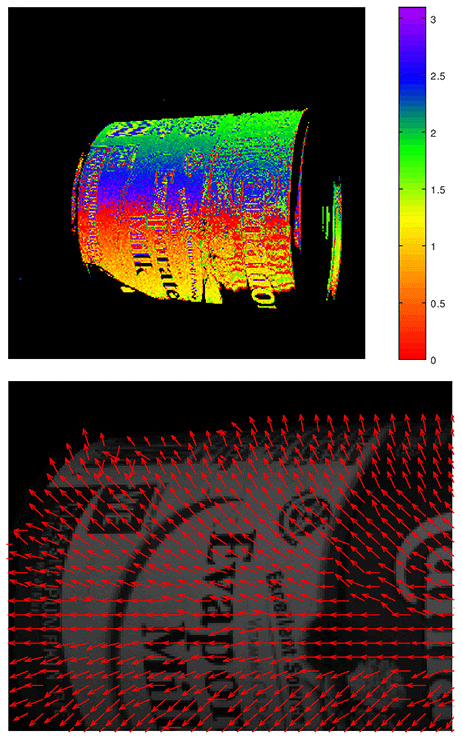
\includegraphics[width=\linewidth]{images/polarization_normals.png}
    \caption{Angle of orientation and estimated surface normals from polarized light \cite{lucidvisionlabs3DDepthSurface2021}}.
    \label{fig:polarization}
\end{figure}






\subsection{Code closer to Problem formulation}
There is a significant difference between how the problem is formulated in the paper and how